\section{Design Catalogue}
\label{sec:catalogue}

The seven candidates at the recommended length, $L/D = 4.5$ ($L = \SI{810}{mm}$), each with the
\SI{60}{mm} shoulder: to scale with the 3U (Figure~\ref{fig:gallery}), flow at $M = 1.4$
(Figure~\ref{fig:fields}) and numbers (Table~\ref{tab:catalogue}, wave drag from the direct runs at
$L/D = 4.5$).

\begin{figure}[tbp]
\centering
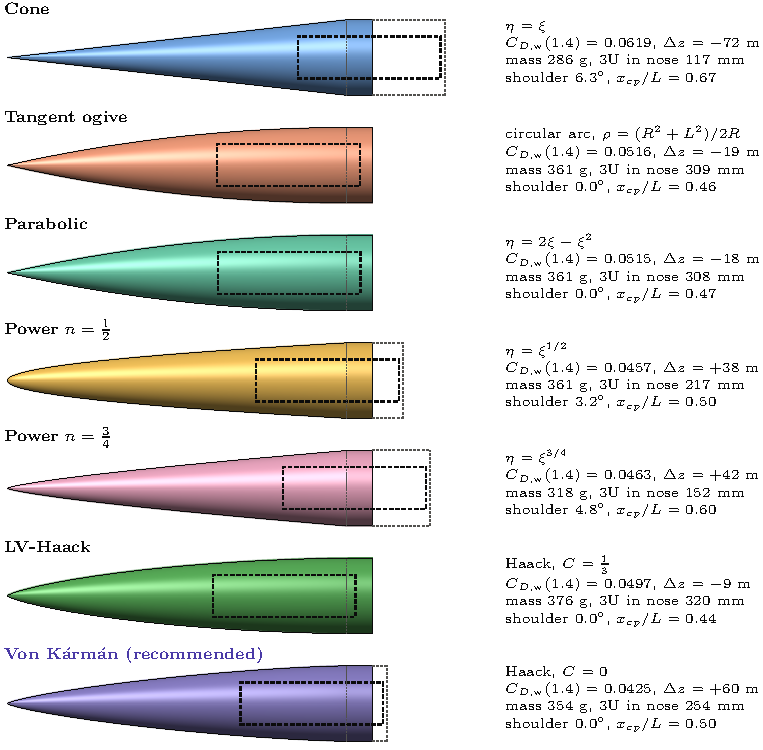
\includegraphics[width=\textwidth]{fig_gallery}
\caption{The seven designs at $L/D=4.5$, rendered to the same scale (diameter \SI{180}{mm}). Thin
dotted line: end of the curved part; dashed box: 3U CubeSat ($100\times100\times\SI{340.5}{mm}$)
pushed forward until its corners reach $r = \SI{77}{mm}$; dotted extension: payload-bay cylinder
still needed behind the \SI{60}{mm} shoulder. $\Delta z$: apogee change relative to the
LVS-length baseline (Von K\'arm\'an at $L/D=4$).}
\label{fig:gallery}
\end{figure}

\begin{figure}[tbp]
\centering
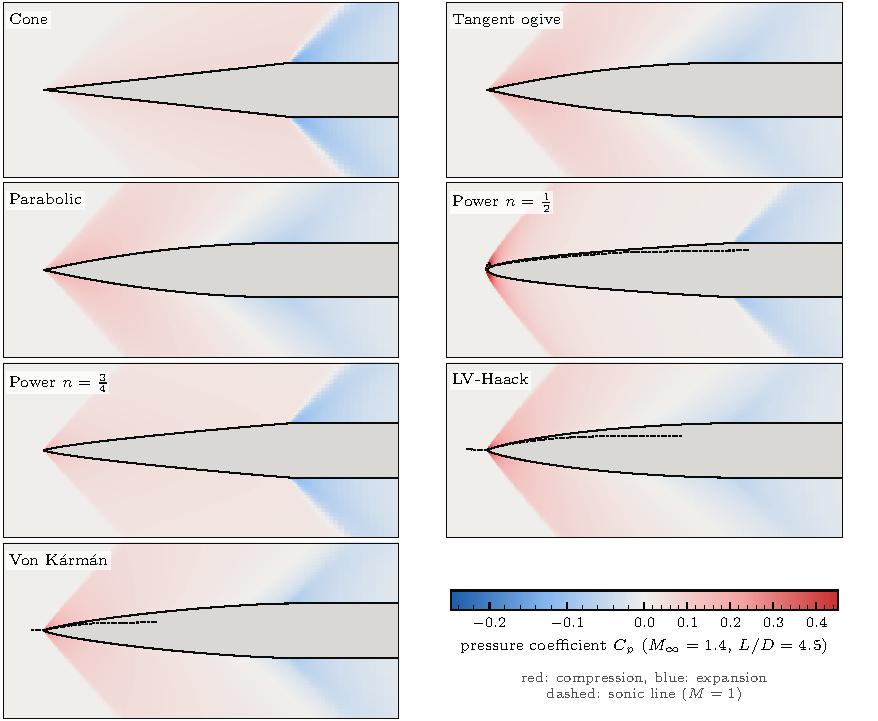
\includegraphics[width=\textwidth]{fig_fields_M14}
\caption{Pressure coefficient around the seven designs at $M_\infty = 1.4$, $L/D = 4.5$
(axisymmetric Euler, mirrored about the axis). The bow shock is the edge of the red region; the
blue fans are the expansions that turn the flow back along the cylinder. The dashed line marks
the sonic line where a subsonic region exists.}
\label{fig:fields}
\end{figure}

In Figure~\ref{fig:fields} the shock leans back at about the Mach angle (Equation~\eqref{eq:mach}); the
cone and power noses expand in one fan at the shoulder kink, the tangent profiles along their aft part.
The more red and the less blue on the nose, the higher the wave drag.

\begin{itemize}[leftmargin=*,itemsep=3pt]
\item \textbf{Conical -- rejected.} Smallest volume (\SI{6.9}{L}) and shell (\SI{286}{g}), simplest mould,
$6.3^\circ$ kink; highest wave drag at every Mach number (46\,\% above Von K\'arm\'an at $M=1.4$). Only
\SI{117}{mm} of the 3U inside (bay \SI{1043}{mm}); $-\SI{132}{m}$ against Von K\'arm\'an.
\item \textbf{Tangent ogive -- acceptable alternative for volume-driven designs.} Bella Lui~II and Nordend
nose, tangent shoulder; 21\,\% more wave drag than Von K\'arm\'an at $M=1.4$. Packages well (\SI{309}{mm}
of the 3U inside, bay \SI{870}{mm}) and is the easiest smooth profile to make, but costs \SI{79}{m}
(about \SI{0.55}{kg}) for \SI{37}{mm} less bay.
\item \textbf{Parabolic ($K' = 1$) -- same as the ogive} (wave drag within 0.4\,\%). Crowell rates it best
in the high subsonic range (Table~\ref{tab:crowell}), irrelevant at $M = 0.8$--1.5.
\item \textbf{Power $n = \tfrac12$ (Wildhorn, Firehorn) -- the choice for a short nose.} Same volume as
Von K\'arm\'an (\SI{10.3}{L}), $3.2^\circ$ kink; its blunt apex gives the only closed sonic line of
Figure~\ref{fig:fields}. Wave drag 3--10\,\% above Von K\'arm\'an at $L/D=4.5$, but the lowest at
$L/D = 3$ and at $M \leq 1.1$ for $L/D = 4$. \SI{217}{mm} of the 3U inside (bay \SI{943}{mm});
\SI{22}{m} below Von K\'arm\'an (about \SI{0.15}{kg}), within \SI{31}{m} in every robustness scenario.
\item \textbf{Power $n = \tfrac34$ -- not selected.} Pointed, slender, small volume (\SI{8.2}{L}),
$4.8^\circ$ kink. Its wave drag falls fastest with Mach ($0.0513 \rightarrow 0.0432$ from $M = 1.2$ to
1.6) and it ends only \SI{18}{m} below Von K\'arm\'an, but has the worst packaging (\SI{152}{mm} of the 3U
inside, bay \SI{1008}{mm}); it suits a faster vehicle ($M_{\max} \approx 2$) with the payload elsewhere.
\item \textbf{LV-Haack ($C = \tfrac13$) -- the choice if payload volume were the driver.} Minimum wave drag
for a given length and volume: fullest (\SI{11.6}{L}), tangent shoulder, 13--19\,\% more wave drag than
Von K\'arm\'an over $M = 1.2$--1.6. Best payload room (\SI{320}{mm} inside, bay \SI{870}{mm}), heaviest
shell (\SI{376}{g}), largest static-margin reduction ($-0.08$ cal); costs \SI{69}{m}.
\item \textbf{Von K\'arm\'an ($C = 0$) -- recommended.} Minimum wave drag for a given length and base area:
thin near the tip, area growth spread along the length. \SI{10.3}{L}, tangent shoulder, $x_{cp}/L = 0.5$;
weak compression at the tip and $C_p < 0$ over the aft third. Lowest wave drag at every computed Mach
number at $L/D = 4.5$ (0.0437, 0.0425, 0.0414 at $M = 1.2$, 1.4, 1.6; $+0.5$ to $+1.4\,\%$ with the
\SI{4.5}{mm} tip). \SI{254}{mm} of the 3U inside (bay \SI{907}{mm}), clean bond line, highest in all seven
robustness scenarios.
\end{itemize}

\begin{table}[H]
\centering
\caption{Design catalogue at $L/D = 4.5$ ($L = \SI{810}{mm}$). Wave drag from the direct Euler runs at this fineness; $\Delta z$ relative to Von K\'arm\'an at $L/D=4$ (LVS length), including length and mass effects.}
\label{tab:catalogue}
\small
\begin{adjustbox}{max width=\textwidth}
\begin{tabular}{@{}lccccccc@{}}
\toprule
 & Cone & Ogive & Parabolic & Power $\tfrac12$ & Power $\tfrac34$ & LV-Haack & Von K\'arm\'an \\
\midrule
Volume [L] & 6.87 & 11.03 & 10.99 & 10.31 & 8.24 & 11.59 & 10.31 \\
Wetted area [m$^2$] & 0.230 & 0.308 & 0.307 & 0.307 & 0.263 & 0.322 & 0.300 \\
Tip semi-angle [$^\circ$] & 6 & 13 & 13 & 89 & 74 & 80 & 78 \\
Shoulder angle [$^\circ$] & 6.3 & 0.0 & 0.0 & 3.2 & 4.8 & 0.0 & 0.0 \\
$x_{cp}/L$ (Barrowman) & 0.667 & 0.465 & 0.467 & 0.500 & 0.600 & 0.438 & 0.500 \\
\midrule
$C_{D,\rm w}$ at $M=1.2$ & 0.0708 & 0.0530 & 0.0529 & 0.0450 & 0.0513 & 0.0496 & 0.0437 \\
$C_{D,\rm w}$ at $M=1.4$ & 0.0619 & 0.0516 & 0.0515 & 0.0457 & 0.0463 & 0.0497 & 0.0425 \\
$C_{D,\rm w}$ at $M=1.6$ & 0.0567 & 0.0504 & 0.0502 & 0.0456 & 0.0432 & 0.0491 & 0.0414 \\
\midrule
$\Delta z$ at $L/D=4$ [m] & -195 & -93 & -92 & -8 & -26 & -75 & +0 \\
$\Delta z$ at $L/D=4.5$ [m] & -72 & -19 & -18 & +38 & +42 & -9 & +60 \\
$\Delta z$ at $L/D=5$ [m] & -23 & +32 & +39 & +75 & +99 & +36 & +99 \\
\midrule
Shell + tip mass [g] & 286 & 361 & 361 & 361 & 318 & 376 & 354 \\
3U inside nose [mm] & 117 & 309 & 308 & 217 & 152 & 320 & 254 \\
Nose-bay length [mm] & 1043 & 870 & 870 & 943 & 1008 & 870 & 907 \\
$\Delta$ static margin [cal] & +0.09 & -0.07 & -0.06 & -0.03 & +0.04 & -0.08 & -0.04 \\
\bottomrule
\end{tabular}
\end{adjustbox}
\end{table}


\subsection{Literature cross-check}
\label{sec:crowell}

Crowell's drag-rating chart (Wikipedia ``Nose cone design'', CC BY-SA 4.0, used in the Firehorn DJF) is an
independent, coarse check (Table~\ref{tab:crowell}; its fineness ratio is not stated).

\begin{table}[H]
\centering
\caption{Crowell's qualitative drag ratings (1 superior, 2 good, 3 fair, 4 inferior; --: no data),
read from the vector chart \texttt{Nose\_cone\_drag\_comparison.svg} (G.\,A. Crowell / C.\,M.\,G.
Lee). Compared with the ranking computed here at $L/D=3$ and $L/D=4.5$.}
\label{tab:crowell}
\small
\begin{tabular}{@{}lccccc|cc@{}}
\toprule
 & \multicolumn{5}{c|}{Crowell rating at $M =$} & \multicolumn{2}{c}{Euler rank at $M=1.4$} \\
Shape & 0.9 & 1.0 & 1.2 & 1.5 & 1.85 & $L/D=3$ & $L/D=4.5$ \\
\midrule
Cone & 4 & 4 & 4 & 4 & 4 & 6 & 7 \\
Tangent ogive & 4 & 4 & 4 & 4 & 4 & 5 & 6 \\
Parabola & 1 & 3 & -- & -- & -- & 4 & 5 \\
Power $\tfrac12$ & 1 & 2 & 2 & 2 & 3 & 1 & 2 \\
Power $\tfrac34$ & 2 & -- & -- & 3 & 2 & -- & 3 \\
LV-Haack & 1 & 1 & -- & -- & -- & 3 & 4 \\
Von K\'arm\'an & 1 & 1 & 1 & 3 & 2 & 2 & 1 \\
\bottomrule
\end{tabular}
\end{table}

Both rate the cone and ogive worst and the Von K\'arm\'an, Haack and power noses good. Around $M = 1.5$ the
chart prefers power $\tfrac12$, which the Euler results reproduce at $L/D = 3$ but not at $L/D \geq 4$: the
ranking depends on fineness, so the recommendation rests on the computed ranking at the design fineness.
